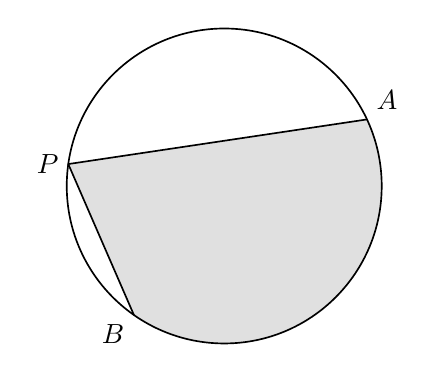
\begin{tikzpicture}[baseline,line cap=round,line join=round,>=stealth]
  \coordinate (O) at (0,0);
  \def\R{2.0}
  \def\angA{25}
  \def\angB{-125}
  \def\angP{172}

  \coordinate (A) at (\angA:\R);
  \coordinate (B) at (\angB:\R);
  \coordinate (P) at (\angP:\R);

  % Shaded region
  \fill[black!12] (P) -- (A) arc(\angA:\angB:\R) -- (B) -- cycle;

  % Circle and segments
  \draw[line width=0.6pt] (O) circle (\R);
  \draw[line width=0.6pt] (P) -- (A);
  \draw[line width=0.6pt] (P) -- (B);

  % Labels
  \node[left] at (P) {$P$};
  \node[above right] at (A) {$A$};
  \node[below left] at (B) {$B$};
\end{tikzpicture}
